\chapter{Application development}
\lhead{Chapter 3 \emph{Application development}}
\label{chap:3}
%\autoref{chap:3}
\bigskip

The mitigation of the overpopulation problem is nowadays an absolute necessity. The application, which is described below, has been developed towards this direction. More specifically, it can give the incentives to create space traffic management rules based on the orbit and capacity allocation, as well as the added value that each new satellite has.

The application has two major capabilities. The first one is the calculation of the revisit time of a single satellite or constellation (Section \ref{revisit time}). The second one is a tool, with which the user can find out what is the added value of an object based on the number of the satellites that are already in-orbit and have the same characteristics (Section \ref{added value}). This tool, in essence, has many more capabilities, which are presented in Chapter \ref{chap:4}.

\bigskip
\section{From satellite definition to revisit time calculation}
\label{revisit time}
\bigskip

The implementation of this first part of the application was programmed and carried out in Python. In this stage, the user defines a satellite by providing its two-line elements (TLE). However, since the application is focused only on the Earth Observation satellites, parameters related to this field are also necessary to be given.
%Write epigrammatika all the different steps here.

\bigskip
\subsection{Necessary input data}
\bigskip

In this first step, the user can define a satellite by providing the TLE set to the application. Despite the fact that the classical orbital elements are used in the scientific community, it was decided that the TLE set is a more convenient and fast way of importing and handling the input data, since the latter way is applied universally and the orbit computation in the next step can be done without any further conversions of those given parameters.

From the elements of a TLE set, eight parameters are being extracted and used in the application. Those are the epoch date, inclination ($i$), Right Ascension of the Ascending Node (RAAN) ($\Omega$), eccentricity ($e$), argument of perigee ($\omega$), mean anomaly ($M$), mean motion ($n$) and the international designator, which is a unique code of a satellite. In the Figure \ref{tle}, it can be seen an example dataset with all the information that TLE carries.

More specifically, the epoch date is the number of days passed in the particular year. The information about the year is taken from the first two digits of the parameter and from the following digits the exact month, day, epoch hour, minute and second can be found. Finally, the epoch time is calculated in seconds as:

\begin{equation}
\label{epoch}
\text{epoch} = (\text{epoch hour} * 3600) + (\text{epoch min} * 60) + \text{epoch sec}.
\end{equation}

\begin{figure}
\centering
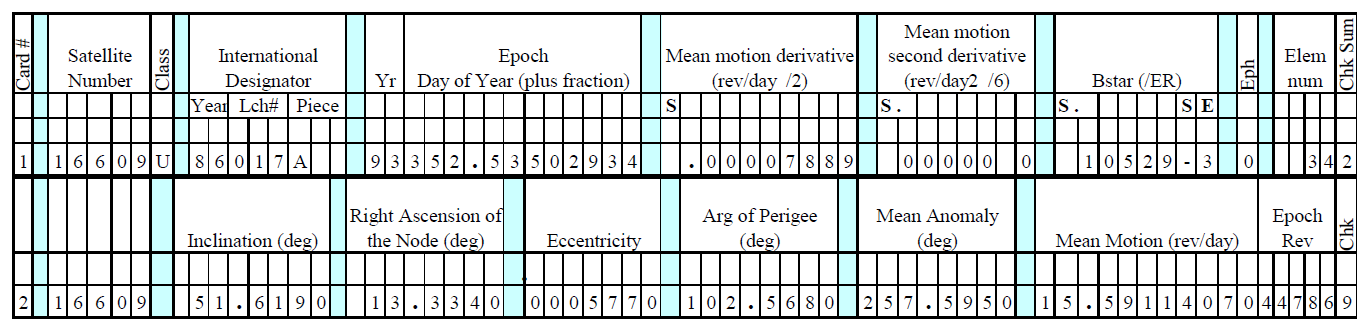
\includegraphics[width=0.9\textwidth]{Images/tle.png}\caption{An example two-line element (TLE) set. S is the sign of values, and E is of exponent. \textit{Source: \cite{Vallado}}}
\label{tle} 
\end{figure}

The parameters of eccentricity, inclination, RAAN, argument of perigee and mean anomaly can be seen graphically in the Figure \ref{keplerian_elements}. In short, eccentricity is a constant defining the shape of the orbit. There is a circular orbit when it is zero and an elliptical orbit when the number is less than one. To the given value of eccentricity from the TLE, a decimal at the beginning must be applied. As far as the inclination, which is given in degrees, it is the angle between the equator and the orbit plane. The RAAN or else the node (degrees) is the angle between vernal equinox and the point where the orbit crosses the equatorial plane and goes towards the north. Argument of perigee is the angle between the ascending node and the orbit's point of the closest approach to the earth, which is called perigee. It is given in degrees. Finally, the mean anomaly is the angle of satellite location in the nominal orbit, which referenced to a circular orbit with radius equal to the semi-major axis. It is measured from the perigee and it is also given in degrees. It should be also noted that the conversion of their units from degrees to radians is necessary, since many other computations will be followed. \cite{Vallado}

From the parameter of mean motion ($n$), the semi-major axis ($a$), as well as the period ($T$) of the orbit can be found. Namely, the mean motion is converted from the unit of $revolutions/day$ to $radian/sec$. Then, the semi-major axis is calculated from the Kepler's 3\textsuperscript{nd} law:
\begin{equation}
\label{3rd_keplers_law}
n^2 a^3 = \mu,
\end{equation}
%a = (\frac{\mu}{n^2})^{1/3},
with $\mu$ being the geometric gravitational parameter.

\begin{figure}
\centering
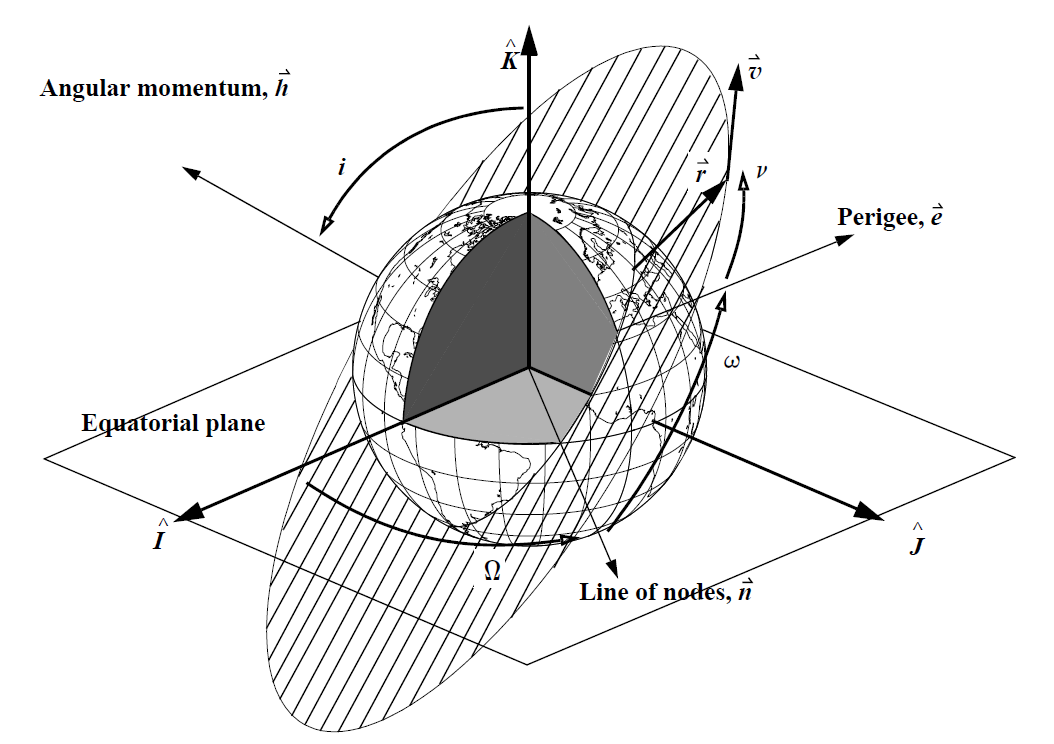
\includegraphics[width=0.9\textwidth]{Images/keplerian_elements.png}\caption{The classical orbital elements: semi-major axis ($a$), eccentricty ($e$), inclination ($i$), Right Ascension of the Ascending Node (RAAN) ($\Omega$), argument of perigee ($\omega$), and true anomaly ($\nu$). \textit{Source: \cite{Vallado}}}
\label{keplerian_elements} 
\end{figure}

Apart from the parameters that were just mentioned, it is necessary to be added some parameters related to the Earth Observation sensor that the satellite has. The orbit lifetime, the type of sensor (see Section \ref{EO}) and the spatial resolution are some of them. However, the determiner parameter in the calculation of the revisit time is the information of the swath width of the sensor, which is inserted in the units of kilometers. Swath is called the area of the Earth that is captured on the image and thus the bigger the number of swath is, the larger the area that is captured. In the Figure \ref{swath_width}, both the swath width and the spatial resolution are illustrated.

\begin{figure}
\centering
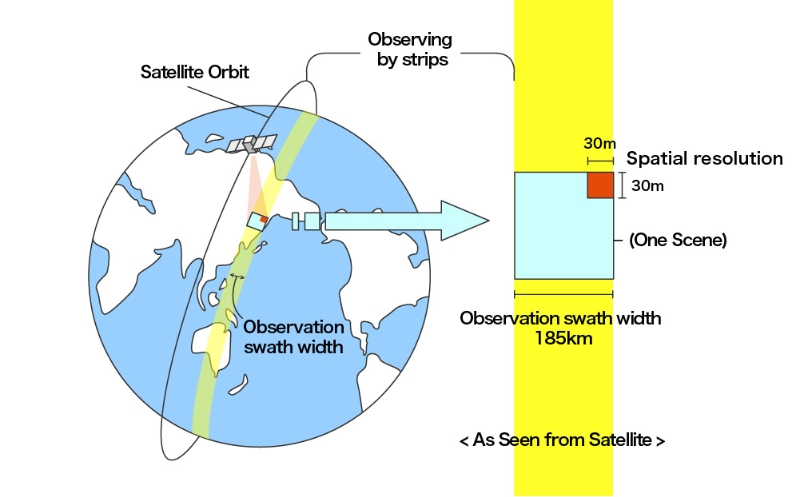
\includegraphics[width=0.9\textwidth]{Images/swath_width.png}\caption{Illustration showing the difference between swath width and spatial resolution. \textit{Source: Remote Sensing Technology Center of Japan - EO in Japan. Website: restec.or.jp (Accessed: October, 2020)}} %https://www.restec.or.jp/en/knowledge/sensing/sensing-3.html
\label{swath_width} 
\end{figure}

\bigskip
\subsection{Orbit computation}
\bigskip

The next step is the computation of the orbit. The imported parameters are given in a geocentric reference system and they define a unique orbit.

\bigskip
\subsubsection{Polar coordinates in orbital plane}
\bigskip

Firstly, the polar coordinates, which are the radius ($r$) and the true anomaly ($v$) are calculated. For this calculation though, the eccentric anomaly ($E$) needs to be found through this transcendental Kepler's equation:
\begin{equation}
E - e \sin{E} = M,
\end{equation}

where $M$ is the mean anomaly. Once the equation has be solved iteratively, the radius ($r$) and true anomaly ($v$) can be found.
\begin{equation}
r = a(1 - e \cos{E}),
\end{equation}

\begin{equation}
\tan{\frac{\nu}{2}} = \sqrt{\frac{1 + e}{1 - e}} \tan{\frac{E}{2}}.
\end{equation}

\bigskip
\subsubsection{Position \& velocity in space-fixed system}
\bigskip

The main idea of this task is the rotation of the orbital plane into the equatorial coordinate system. The angles that were used to the rotation matrices were the RAAN ($\Omega$), the inclination ($i$), and the argument of perigee ($\omega$). In the Figure \ref{orbit_to_space}, the rotation of the orbital plane is illustrated based on the aforementioned angles. For achieving that, the position (Equation \ref{position_orbital}) and velocity (Equation \ref{velocity_orbital}) in the orbital plane should be calculated first \cite{Montenbruck}:

\begin{figure}
\centering
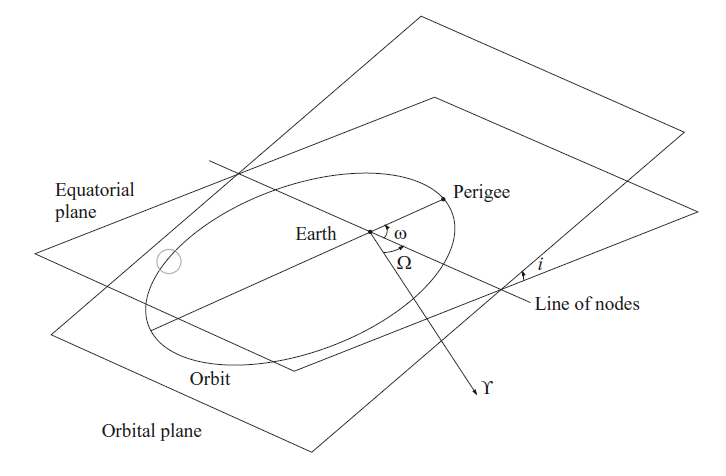
\includegraphics[width=0.9\textwidth]{Images/orbit_to_space.png}\caption{The rotation of the orbital plane into the equatorial plane with the help of the following orbital elements of the satellite: inclination ($i$), RAAN ($\Omega$) and argument of perigee ($\omega$). \textit{Source: \cite{Montenbruck}}}
\label{orbit_to_space} 
\end{figure}

\begin{equation}
\label{position_orbital}
\vv{r_{b}} = r \begin{bmatrix} \cos{v} \\ \sin{v} \\ 0 \end{bmatrix}
\end{equation}
\begin{equation}
\label{velocity_orbital}
\dot{\vv{r_{b}}} = \sqrt{\frac{\mu}{a (1 - e^2)}} \begin{bmatrix} -\sin{v} \\ e + \cos{v} \\ 0 \end{bmatrix},
\end{equation}

where $\mu$ the geometric gravitational parameter (Equation \ref{3rd_keplers_law}).

Then, the position and the velocity in the space-fixed system are found through \cite{Montenbruck}:
\begin{equation}
\label{space-fixed}
\vv{r} = R_3 (-\Omega) R_1  (-i) R_3 (-\omega) \vv{r_{b}},
\end{equation}
\begin{equation}
\dot{\vv{r}} = R_3 (-\Omega) R_1  (-i) R_3 (-\omega) \dot{\vv{r_{b}}},
\end{equation}
where $\vv{r_{b}}$, $\dot{\vv{r_{b}}}$ are taken from the equations \ref{position_orbital}, \ref{velocity_orbital} respectively. The elementary matrices that were used are:
\begin{equation}
R_1(\theta) = \begin{bmatrix} 1 & 0 & 0 \\ 0 & \cos{\theta} & \sin{\theta} \\ 0 & -\sin{\theta} & \cos{\theta} \end{bmatrix},
\end{equation}
for the rotation around the x-axis ($R_{1}$), and
\begin{equation}
\label{R3}
R_3(\theta) = \begin{bmatrix} \cos{\theta} & \sin{\theta} & 0 \\ -\sin{\theta} & \cos{\theta} & 0 \\ 0 & 0 & 1 \end{bmatrix},
\end{equation}
for the rotation around z-axis ($R_{3}$) \cite{Montenbruck}.

\bigskip
\subsubsection{Position \& velocity in earth-fixed system}
\bigskip

After the orbit calculation in the space-fixed system, the position and velocity in the earth-fixed system can be found. Based on the rotation rate of the Earth ($\Omega_{E}$) and the sidereal angle, the angle of rotation ($\theta_{0}$) (Equation \ref{theta_angle}) between the space and earth system is calculated. The sidereal angle is calculated through the Greenwich mean sidereal time \cite{Vallado}, having as an input the Julian date from the information about the epoch time (Equation \ref{epoch}).

\begin{equation}
\label{rotation_rate}
\Omega_{E} = \frac{2 \pi}{86164}
\end{equation}

\begin{equation}
\label{theta_angle}
\theta_{0}(t) = \Omega_{E} \cdot t + \text{sidereal angle}
\end{equation}

Both angles, the angle of rotation $\theta_{0}$ and the sidereal angle, should be in radian in order to be used in the following steps. Finally, the position in the earth-fixed system is calculated using the rotation matrix around the z-axis (Equation \ref{R3}) as:
\begin{equation}
\vv{r}_{Earth-fixed}(t) = R_{3}(\theta_{0}(t)) \vv{r},
\end{equation}
where $\vv{r}$ is the position in the space-fixed system (Equation \ref{space-fixed}).

\bigskip
\subsubsection{Longitude \& latitude on the Earth's surface}
\bigskip

In order to calculate the position of the sub-satellite's points on the Earth's surface, the longitude and latitude is needed. The equations that link the Earth-fixed coordinates with the $\lambda$ and $\phi$ are the following:

\begin{equation}
\tan{\lambda} = \frac{y_{\text{Earth-fixed}}}{x_{\text{Earth-fixed}}},
\end{equation}

\begin{equation}
\tan{\phi} = \frac{z_{\text{Earth-fixed}}}{\sqrt{x^2_{\text{Earth-fixed}} + y^2_{\text{Earth-fixed}}}}.
\end{equation}

The groundtrack of the orbit, which is the path of the sub-satellite point as the satellite travels through its orbit, can be consequently acquired. However, the actual groundtrack of a satellite differs from a simple circle that results from the intersection of the orbital plane with the surface of the Earth. For a satellite with a period $T$, the longitude $\lambda$ is shifted from one revolution to the next \cite{Montenbruck} :
\begin{equation}
\Delta \lambda_{\Omega} = - \dot{\theta} \cdot T = - 0.2507^{\circ}/ min \cdot T,
\end{equation}

where $\dot{\theta}$ is the Greenwich mean sidereal at time $t$. This is due to the Earth's rotation, as it can be seen in the Figure \ref{groundtrack-fixed-rotating}.

\begin{figure}
\centering
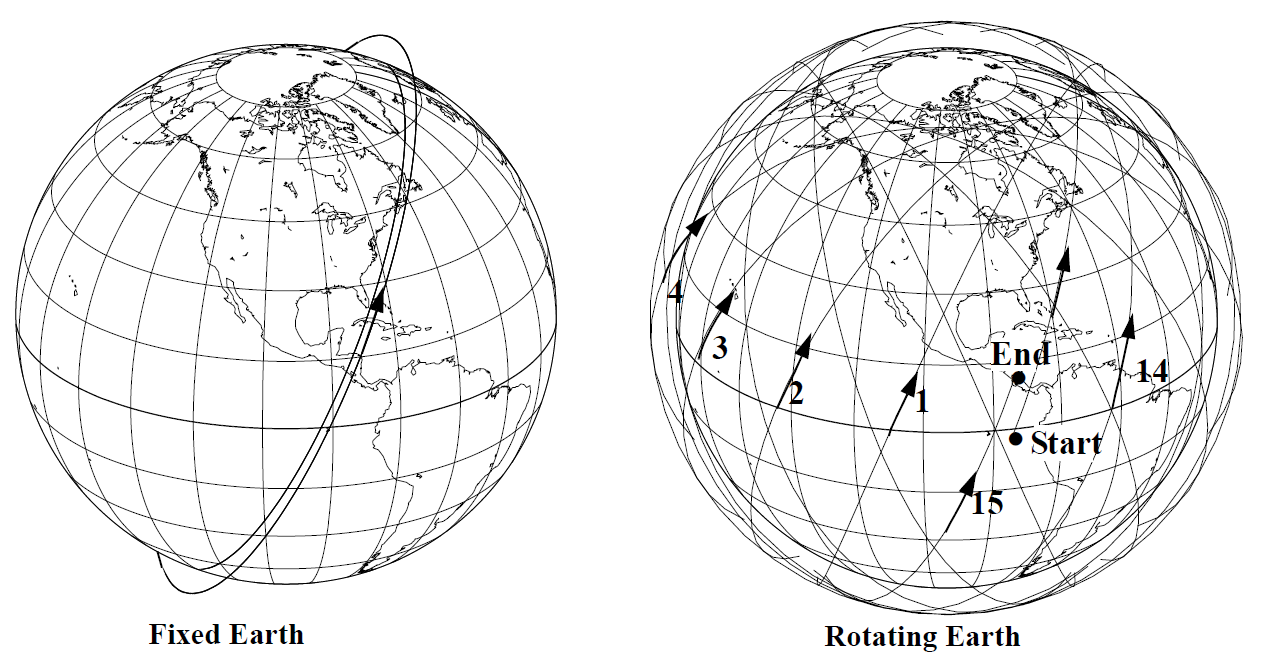
\includegraphics[width=0.9\textwidth]{Images/groundtrack-fixed-rotating.png}\caption{Illustration of the groundtracks in cases where the Earth is fixed and rotating. \textit{Source: \cite{Vallado}}}
\label{groundtrack-fixed-rotating} 
\end{figure}

\bigskip
\subsubsection{Perturbation on the orbital elements}
\bigskip

Since the focus of this application is on the low earth orbit (LEO) satellites, the gravity field is the largest perturbation, which cause secular motion to some of the orbital elements. The RAAN is one the affected by the zonal harmonics, and the equation that describes it:
\begin{equation}
\dot{\Omega} = - \frac{3 n R_{\bigoplus}^{2} J_{2} \cos{i}}{2 a^{2}},
\end{equation}
where $R_{\bigoplus}$ is the radius of the Earth according to WGS-84 (6378.137 km), and as $n$ the mean motion is used \cite{Montenbruck}.

Due to secular perturbations, the argument of perigee is also affected:
\begin{equation}
\dot{\omega} = - \frac{3 n R_{\bigoplus}^{2} J_{2}}{4 a^{2}} (1 - 5 \cos^{2}{i}).
\end{equation}

% Vallado p. 674 + Montenbruck p.50

\bigskip
\subsubsection{Revisit time definition}
\bigskip


% Define revisit time --> average (median) revisit time in equator
%ABOUT REVISIT TIME:
%The interval of time required for the satellite to complete its orbit cycle is not the same as the "revisit period". Due to the steerable sensors, the off-nadir angles, the large swath width , the revisit time can be less than the orbit cycle time. "The revisit period is an important consideration for a number of monitoring applications, especially when frequent imaging is required (for example, to monitor the spread of an oil spill, or the extent of flooding). In near-polar orbits, areas at high latitudes will be imaged more frequently than the equatorial zone due to the increasing overlap in adjacent swaths as the orbit paths come closer together near the poles." (Source: https://www.nrcan.gc.ca/maps-tools-and-publications/satellite-imagery-and-air-photos/remote-sensing-tutorials/acknowledgements-permission-use/9391)

\subsection{Computational calculation of revisit time}

In order to approach the issue of calculating the revisit time in equator The swath width of the sensor defines somehow the "area". 

\subsubsection{Map projection}

%Print earth map. Based on the FOV and the revisit frequency, I can see how the Earth will be printed/colored (heat map). So, we want to track coverage/ revisit time across the equator.

% Tip: "Do not present data at this stage but use sketches or synthetic data instead"






%(If I want to further analyze about the satellite viewing geometries and scanning patterns: Page 21,22 in http://www.atmosp.physics.utoronto.ca/people/strong/phy499/section2_05.pdf) --> It makes sense to do it if a use different ways to calculate the revisit time. So, if for every satellite I have the detailed info about the viewing geometry then I can do it. Another way is to write those info in the theory part and then calculate the revisit time, since I don't have much info ...

%As far as the Space-Time Sampling in the LEO satellites: a) sampling is highly dependent on the orbit, b) area viewed on one orbit overlaps area viewed on the previous and succeeding orbits, c) usually view every point on the Earth twice a day, d) view each point a small number of local times but at varying elevation and azimuth angles.

\bigskip
\section{Added value of satellite based on operational similar objects}
\label{added value}
\bigskip

\bigskip
\subsection{Database}
\bigskip
% Mention the focus on LEO and EO satellites
% Implemented in PostgreSQL

%In the chapter, where you will talk about the database, add big tables about the results - with the commercial and non-commercial constellations & then put a reference next to the other table that I have only the commercial EO satellites in the "Chapter_1" (~ Seira 234)!

%\section{Sources of data}
%\bigskip
%
%\section{Data gathering procedure}
%\bigskip

\bigskip
\subsection{Classification of Earth Observation field}
\bigskip


% Different import ways of adding data


